
\mode%%%%%%%%%%%%%%%%%%%%%%%%%%%%%%%%%%%%%%%%%
% Beamer Presentation
% LaTeX Template
% Version 1.0 (10/11/12)
%
% This template has been downloaded from:
% http://www.LaTeXTemplates.com
%
% License:
% CC BY-NC-SA 3.0 (http://creativecommons.org/licenses/by-nc-sa/3.0/)
%
%%%%%%%%%%%%%%%%%%%%%%%%%%%%%%%%%%%%%%%%%

%----------------------------------------------------------------------------------------
%	PACKAGES AND THEMES
%----------------------------------------------------------------------------------------

\documentclass{beamer}
\usepackage{booktabs}
\mode<presentation> {


% The Beamer class comes with a number of default slide themes
% which change the colors and layouts of slides. Below this is a list
% of all the themes, uncomment each in turn to see what they look like.

%\usetheme{default}
%\usetheme{AnnArbor}
%\usetheme{Antibes}
%\usetheme{Bergen}
%\usetheme{Berkeley}
%\usetheme{Berlin}
%\usetheme{Boadilla}
%\usetheme{CambridgeUS}
%\usetheme{Copenhagen}
%\usetheme{Darmstadt}
%\usetheme{Dresden}
%\usetheme{Frankfurt}
%\usetheme{Goettingen}
%\usetheme{Hannover}
%\usetheme{Ilmenau}
%\usetheme{JuanLesPins}
%\usetheme{Luebeck}
\usetheme{Madrid}
%\usetheme{Malmoe}
%\usetheme{Marburg}
%\usetheme{Montpellier}
%\usetheme{PaloAlto}
%\usetheme{Pittsburgh}
%\usetheme{Rochester}
%\usetheme{Singapore}
%\usetheme{Szeged}
%\usetheme{Warsaw}
%\usetheme{LMU}
% As well as themes, the Beamer class has a number of color themes
% for any slide theme. Uncomment each of these in turn to see how it
% changes the colors of your current slide theme.

%\usecolortheme{albatross}
\usecolortheme{beaver}
%\usecolortheme{beetle}
%\usecolortheme{crane}
%\usecolortheme{dolphin}
%\usecolortheme{dove}
%\usecolortheme{fly}
%\usecolortheme{lily}
%\usecolortheme{orchid}
%\usecolortheme{rose}
%\usecolortheme{seagull}
%\usecolortheme{seahorse}
%\usecolortheme{whale}
%\usecolortheme{wolverine}

%\setbeamertemplate{footline} % To remove the footer line in all slides uncomment this line
\setbeamertemplate{footline}[page number] % To replace the footer line in all slides with a simple slide count uncomment this line

\setbeamertemplate{navigation symbols}{} % To remove the navigation symbols from the bottom of all slides uncomment this line
}

\usepackage{graphicx}
\usepackage{graphics}% Allows including images
\usepackage{booktabs} % Allows the use of \toprule, \midrule and \bottomrule in tables
\usepackage {tikz}
\usepackage{tkz-graph}
\GraphInit[vstyle = Shade]
\tikzset{
  LabelStyle/.style = { rectangle, rounded corners, draw,
                        minimum width = 2em, fill = yellow!50,
                        text = red, font = \bfseries },
  VertexStyle/.append style = { inner sep=5pt,
                                font = \normalsize\bfseries},
  EdgeStyle/.append style = {->, bend left} }
\usetikzlibrary {positioning}
%\usepackage {xcolor}
\definecolor {processblue}{cmyk}{0.96,0,0,0}
%----------------------------------------------------------------------------------------
%	TITLE PAGE
%----------------------------------------------------------------------------------------

\title[Short title]{Replication of "Critical Recidivsm after Prison and Electronic Monitoring" by Di Tella and Schargrodsky} % The short title appears at the bottom of every slide, the full title is only on the title page

\author{Maripjan Koshmatov \and Bakai Baiazbekov \and Aijing Sun} % Your name
\institute[LMU Munich] % Your institution as it will appear on the bottom of every slide, may be shorthand to save space
{
University of Munich \\ % Your institution for the title page
\medskip
}
\date{\today} % Date, can be changed to a custom date

\begin{document}


\begin{frame}
\titlepage % Print the title page as the first slide
\end{frame}

\begin{frame}
\frametitle{Overview} % Table of contents slide, comment this block out to remove it
\tableofcontents % Throughout your presentation, if you choose to use \section{} and \subsection{} commands, these will automatically be printed on this slide as an overview of your presentation
\end{frame}

%----------------------------------------------------------------------------------------
%	PRESENTATION SLIDES
%--------------------------------------------------------------------
\section{Motivation}
\begin{frame}{Motivation}
\begin{figure}        
\centering
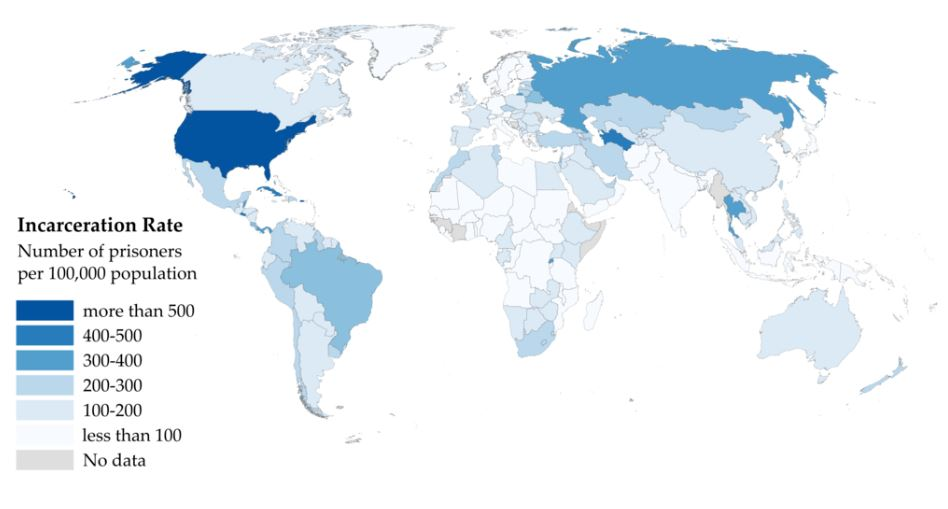
\includegraphics[width=\textwidth]{prison}
\end{figure}
 \end{frame}

%------------------------------------------------
\begin{frame}{Motivation}
    \begin{itemize}
        \item Keeping prisons is very costly (Kuziemko 2013)
        \item Yet, it bears even higher cost if criminals are not isolated from society
        \item On the other hand, given brutality and psychologically destructive effects of prison on individuals, prisons might stimulate people to commit crimes in the future over and over again.
        \item So, are the other punishment tools that is more efficient compared to prison?
    \end{itemize}
\end{frame}
%------------------------------------------------
\begin{frame}{Motivation}
    \begin{itemize}
        \item Probably the most widespread substitution for imprisonment is Electronic Monitoring (EM) of convicted individuals.
\begin{figure}        
\centering
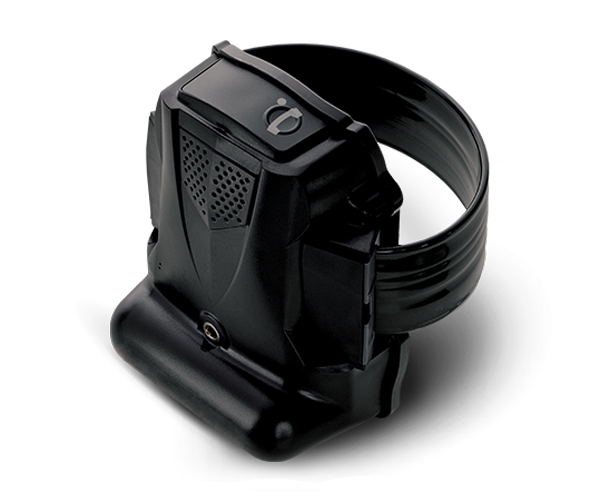
\includegraphics[width=0.3\textwidth]{EM.jpg}
\end{figure}

\item But is it worth to implement EM? What are the risks and who should receive them instead of imprisonment?
\end{itemize}
\end{frame}
%------------------------------------------------
\begin{frame}{Motivation}
   \begin{figure}[t]
\begin{subfigure}
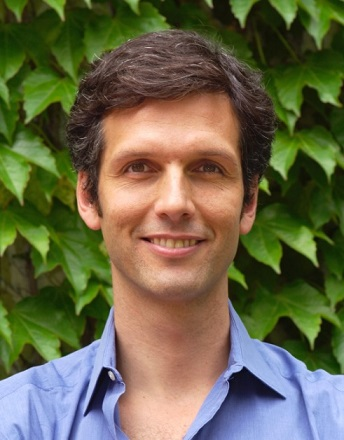
\includegraphics[width=3cm, height=4cm, left]{DiTella.jpg}
\end{subfigure}
\hspace{1.9 cm}
\begin{subfigure}
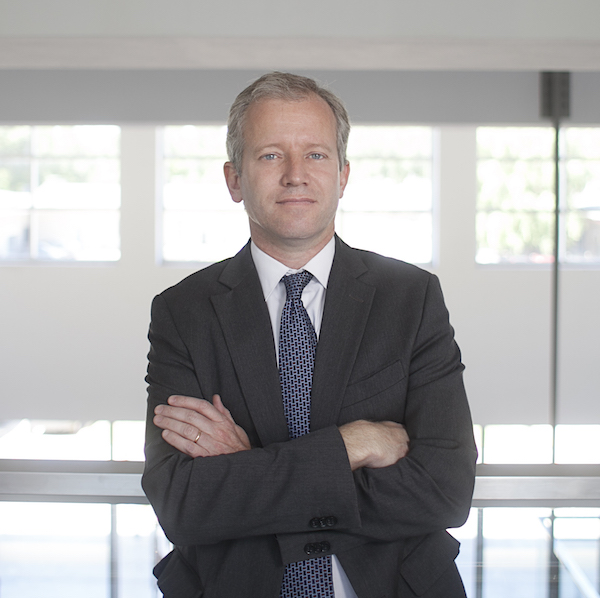
\includegraphics[width=3cm, height=4cm, right]{Ernesto.jpg}
\end{subfigure}        
\end{figure}
 \centerline{Rafael Di Tella \; \;\;\;\;\;\; \;\;\;\;\;\; \;\;\; Ernesto Schargrodsky}   
\begin{center}
 Authors of \textit{"Criminal Recidivism after Electronic Monitoring and Imprisonment"} (JPE, 2013)   
\end{center}
\end{frame}

%------------------------------------------------
\begin{frame}{Summary of the paper}
\begin{itemize}
        \item Aim of study: To contribute to a long-lasting debate of whether EM can be a good alternative for imprisonment
        \item Specifically, is EM a useful tool in reducing recidivism. 
        \item To do that authors compare the outcomes of individuals who received EM vs that of those who were imprisoned.
        \item To estimate the of effect a quasi-experiment was conducted between 1998-2007 in Buenos-Aires Province of Argentine
        
                \end{itemize}
\end{frame}
%------------------------------------------------
\begin{frame}{Summary of the paper}
\begin{itemize}
        \item However, directly comparing the difference of outcomes between offenders treated with electronic monitoring vs those released from  prison is naive. 
        \item Two issues may come into play here:
        \begin{itemize}
        \item  1.Selection Problem
        \item 2.Differential risk of the target
        \end{itemize}
            \end{itemize}
\end{frame}
%------------------------------------------------
\begin{frame} {Summary of the paper}
\begin{itemize}
\item \textit{Selection Problem} was resolved by random assignment of arrested individuals to judges.
\item Judges were assigned to duties randomly.
\item The second problem that might be a source endogeneity will be discussed below
        \end{itemize}
\end{frame}
%------------------------------------------------

\begin{frame}{Summary of the paper}
\begin{itemize}
        \item Authors compare effects of electronic monitoring vs imprisonment on future recidivism
         \begin{equation}
    \centering
    EM_i = \pi_0 + \pi_1Z_{1i} + \pi_2Z_{2i} + \pi_2X_{2i} + ... + \pi_iX_{ij} + u_i  
    \end{equation}
    
        
         \begin{equation}
    \centering
    Recidivism_i = \beta_0 + \beta_1\widehat{EM_i} + \pi_2X_{2i} + ... + \pi_iX_{ij} + u_i  
\end{equation}
        
    \end{itemize}
\end{frame}
%------------------------------------------------
\begin{frame}{Summary of the paper}
\begin{itemize}
        \item Conclusion: There is a significant negative effect on criminal recidivism of treatment individual with electronic monitoring relative to prison. 
        \item According to estimates, assigning convicted individual to EM on average can reduce recidivism risk by that individual between 11-16 percentage points(\textit{ceteris paribus}).
        \item  Here is what authors did.
    \end{itemize}
\end{frame}


%------------------------------------------------
\section{Replication}
\begin{frame}{Data and Replication Tools}
\begin{itemize}
    \item Datasets: Obtained from the University of Chicago website \item Tools used:
    \begin{itemize}
    \item STATA: 14.0 and  15.1 SE
    \item R
    \end{itemize}
    
\end{itemize}
\end{frame}
%------------------------------------------------
\begin{frame}{Replication steps}
 \begin{itemize}
    \item Going through STATA codes to see whether specifications were entered correctly and match those that were described in the paper
    \item Comparison of two estimates
    \item Extraction of results to tables
    \end{itemize}
\end{frame}
%------------------------------------------------
\begin{frame}{Replication tables}

\end{frame}

%------------------------------------------------

\begin{frame}{Replication Tables}
\begin{table}[!htbp] 
  \caption{Electronic Monitoring Assignment and Type of Crimes} 
  \label{Table 2} 
 \resizebox{\linewidth}{!}{
\begin{tabular}{@{\extracolsep{5pt}}lccccc} 
\\[-1.8ex]\hline 
\hline \\[-1.8ex] 
 & \multicolumn{5}{c}{\textit{Dependent variable:}} \\ 
\cline{2-6} 
\\[-1.8ex] & \multicolumn{5}{c}{electronicMonitoring} \\ 
 & (I) & (II) & (III) & (IV) & (V) \\ 
 
\hline \\[-1.8ex] 
 percJudgeSentToEM & 0.663$^{***}$ & 0.660$^{***}$ & 0.660$^{***}$ & 0.660$^{***}$ & 0.637$^{***}$ \\ 
  & (0.085) & (0.085) & (0.085) & (0.085) & (0.087) \\ 
  & & & & & \\ 
 judgeAlreadyUsedEM &  &  &  &  & 0.006$^{**}$ \\ 
  &  &  &  &  & (0.002) \\ 
  & & & & & \\ 
 mostSeriousCrime02 - Attempted homicide &  & $-$0.001 & $-$0.001 & $-$0.001 & $-$0.001 \\ 
  &  & (0.008) & (0.008) & (0.008) & (0.008) \\ 
  & & & & & \\ 
 mostSeriousCrime03 - Sexual offenses &  & 0.001 & 0.001 & 0.0004 & 0.0003 \\ 
  &  & (0.008) & (0.008) & (0.008) & (0.008) \\ 
  & & & & & \\ 
 mostSeriousCrime05 - Aggravated robbery &  & $-$0.004 & $-$0.003 & $-$0.003 & $-$0.003 \\ 
  &  & (0.004) & (0.004) & (0.004) & (0.004) \\ 
  & & & & & \\ 
 
 age &  &  &  & $-$0.00001$^{**}$ & $-$0.00001$^{*}$ \\ 
  &  &  &  & (0.00000) & (0.00000) \\ 
  & & & & & \\ 

 numberPreviousImprisonments &  &  & $-$0.004$^{***}$ & $-$0.005$^{***}$ & $-$0.005$^{***}$ \\ 
  &  &  & (0.001) & (0.001) & (0.001) \\ 
  & & & & & \\ 
 yearOfImprisonment &  &  &  & 0.001$^{***}$ & 0.001$^{***}$ \\ 
  &  &  &  & (0.0004) & (0.0004) \\ 
  & & & & & \\ 
  
 Constant & 0.003 & 0.009 & 0.010 & $-$2.677$^{***}$ & $-$2.389$^{***}$ \\ 
  & (0.005) & (0.006) & (0.006) & (0.728) & (0.722) \\ 
  & & & & & \\ 
\hline \\[-1.8ex] 
Observations & 24,003 & 24,003 & 24,003 & 23,928 & 23,928 \\ 
R$^{2}$ & 0.043 & 0.044 & 0.045 & 0.046 & 0.046 \\ 
Adjusted R$^{2}$ & 0.042 & 0.043 & 0.043 & 0.045 & 0.045 \\ 
Residual Std. Error & 0.122 (df = 23984) & 0.122 (df = 23974) & 0.122 (df = 23973) & 0.122 (df = 23894) & 0.122 (df = 23893) \\ 
F Statistic & 59.209$^{***}$ (df = 18; 23984) & 39.347$^{***}$ (df = 28; 23974) & 38.579$^{***}$ (df = 29; 23973) & 34.821$^{***}$ (df = 33; 23894) & 34.054$^{***}$ (df = 34; 23893) \\ 
\endrule
\hline 
\hline \\[-1.8ex] 
\textit{Note:}  & \multicolumn{5}{r}{$^{*}$p$<$0.1; $^{**}$p$<$0.05; $^{***}$p$<$0.01} \\ 
\end{tabular} }
\end{table} 

\end{frame}

%------------------------------------------------
\begin{frame}{Replication tables}
\begin{table}[!htbp] 
  \caption{Recidivism and Electronic Monitoring OLS Regressions} 
  \label{} 
  \resizebox{\columnwidth}{!}{
\begin{tabular}{@{\extracolsep{5pt}}lccccc} 
\\[-1.8ex]\hline 
\hline \\[-1.8ex] 
 & \multicolumn{5}{c}{\textit{Dependent variable:}} \\ 
\cline{2-6} 
\\[-1.8ex] & \multicolumn{5}{c}{recidivism} \\ 
\\[-1.8ex] & \multicolumn{2}{c}{\textit{OLS}} & \textit{probit} & \multicolumn{2}{c}{\textit{OLS}} \\ 
 & (I) & (II) & (III) & (IV) & (V) \\ 

\hline \\[-1.8ex] 
 electronicMonitoring & $-$0.092$^{***}$ & $-$0.090$^{***}$ & $-$0.405$^{***}$ & $-$0.089$^{***}$ & $-$0.086$^{***}$ \\ 
  & (0.021) & (0.024) & (0.107) & (0.024) & (0.023) \\ 
  & & & & & \\ 
 judgeEverUsedEM &  &  &  &  & $-$0.017 \\ 
  &  &  &  &  & (0.024) \\ 
  & & & & & \\ 
 mostSeriousCrime02 - Attempted homicide &  & 0.010 &  & 0.011 & 0.011 \\ 
  &  & (0.064) &  & (0.064) & (0.063) \\ 
  & & & & & \\ 
 mostSeriousCrime03 - Sexual offenses &  & $-$0.038 &  & $-$0.045 & $-$0.029 \\ 
  &  & (0.052) &  & (0.052) & (0.050) \\ 
  & & & & & \\ 

 numberPreviousImprisonments &  & 0.167$^{***}$ & 0.683$^{***}$ & 0.157$^{***}$ & 0.175$^{***}$ \\ 
  &  & (0.024) & (0.089) & (0.024) & (0.024) \\ 
  & & & & & \\ 
 yearOfImprisonment &  & $-$0.058$^{***}$ & $-$0.262$^{***}$ & $-$0.057$^{***}$ &  \\ 
  &  & (0.018) & (0.056) & (0.018) &  \\ 
  & & & & & \\ 

 Constant & 0.224$^{***}$ & 116.588$^{***}$ & 527.711$^{***}$ & 115.193$^{***}$ & 1.622$^{***}$ \\ 
  & (0.012) & (36.256) & (113.254) & (36.845) & (0.305) \\ 
  & & & & & \\ 
\hline \\[-1.8ex] 
Observations & 1,526 & 1,526 & 1,513 & 1,526 & 1,503 \\ 
R$^{2}$ & 0.010 & 0.185 &  & 0.180 & 0.177 \\ 
Adjusted R$^{2}$ & 0.009 & 0.162 &  & 0.158 & 0.163 \\ 
Residual Std. Error & 0.399 (df = 1524) & 0.367 (df = 1484) &  & 0.368 (df = 1485) & 0.368 (df = 1477) \\ 
F Statistic & 15.210$^{***}$ (df = 1; 1524) & 8.212$^{***}$ (df = 41; 1484) &  & 8.154$^{***}$ (df = 40; 1485) & 12.685$^{***}$ (df = 25; 1477) \\ 
\hline 
\hline \\[-1.8ex] 
\textit{Note:}  & \multicolumn{5}{r}{$^{*}$p$<$0.1; $^{**}$p$<$0.05; $^{***}$p$<$0.01} \\ 
\end{tabular} }
\end{table} 
\end{frame}
%------------------------------------------------
\begin{frame}{Replication tables}
\begin{table}[!htbp] \centering 
  \caption{Recidivism and Electronic Monitoring IV regressions} 
  \label{} 
    \resizebox{\columnwidth}{!}{
\begin{tabular}{@{\extracolsep{5pt}}lccccc} 
\\[-1.8ex]\hline 
\hline \\[-1.8ex] 
 & \multicolumn{5}{c}{Dependent Variable: recidivism} \\ 
\cline{2-6} 
 & IV: court & IV: percJudgeSentToEM & IVs: percJudgeSentToEM, judgeAlreadyUsedEM & IV probit & IV: largeSampleEstimate \\ 
\\[-1.8ex] & (1) & (2) & (3) & (4) & (5)\\ 
\hline \\[-1.8ex] 
 EM1\_pred & $-$0.112$^{**}$ &  &  &  &  \\ 
  & (0.057) &  &  &  &  \\ 
  & & & & & \\ 
 EM12\_pred &  & $-$0.138 &  &  &  \\ 
  &  & (0.093) &  &  &  \\ 
  & & & & & \\ 
 EM13\_pred &  &  & $-$0.158$^{*}$ &  & $-$0.158$^{*}$ \\ 
  &  &  & (0.091) &  & (0.091) \\ 
  & & & & & \\ 
 EM14\_pred &  &  &  & $-$0.174$^{*}$ &  \\ 
  &  &  &  & (0.095) &  \\ 
  & & & & & \\ 

 
 Constant & 92.101$^{***}$ & 91.615$^{***}$ & 91.534$^{***}$ & 91.692$^{***}$ & 91.534$^{***}$ \\ 
  & (8.341) & (8.349) & (8.344) & (8.353) & (8.344) \\ 
  & & & & & \\ 
\hline \\[-1.8ex] 
Observations & 1,503 & 1,503 & 1,503 & 1,494 & 1,503 \\ 
R$^{2}$ & 0.168 & 0.167 & 0.167 & 0.167 & 0.167 \\ 
Adjusted R$^{2}$ & 0.149 & 0.148 & 0.148 & 0.148 & 0.148 \\ 
Residual Std. Error & 0.371 (df = 1469) & 0.371 (df = 1469) & 0.371 (df = 1469) & 0.372 (df = 1461) & 0.371 (df = 1469) \\ 
F Statistic & 8.985$^{***}$ (df = 33; 1469) & 8.897$^{***}$ (df = 33; 1469) & 8.924$^{***}$ (df = 33; 1469) & 9.136$^{***}$ (df = 32; 1461) & 8.924$^{***}$ (df = 33; 1469) \\ 
\hline 
\hline \\[-1.8ex] 
\end{tabular} }
\end{table} 
\end{frame}
%------------------------------------------------
\begin{frame}{Replication tables}
\begin{table}[!htbp] 
  \caption{Recidivism and Electronic Monitoring Robustness} 
  \label{} 
      \resizebox{\columnwidth}{!}{
\begin{tabular}{@{\extracolsep{5pt}}lcccc} 
\\[-1.8ex]\hline 
\hline \\[-1.8ex] 
 & \multicolumn{4}{c}{Dependent Variable: recidivism} \\ 
\cline{2-5} 
 & IVs: percJudgeSentToEM, judgeAlreadyUsedEM & IVs: percJudgeSentToEM, judgeAlreadyUsedEM & IVs: percJudgeSentToEM, judgeAlreadyUsedEM & IVs: percJudgeSentToEM, judgeAlreadyUsedEM \\ 
\\[-1.8ex] & (1) & (2) & (3) & (4)\\ 
\hline \\[-1.8ex] 
 EM161\_pred & $-$0.243$^{**}$ &  &  &  \\ 
  & (0.105) &  &  &  \\ 
  & & & & \\ 
 EM162\_pred &  & $-$0.151 &  &  \\ 
  &  & (0.117) &  &  \\ 
  & & & & \\ 
 EM163\_pred &  &  & $-$0.154$^{*}$ &  \\ 
  &  &  & (0.091) &  \\ 
  & & & & \\ 
 EM165\_pred &  &  &  & $-$0.210$^{**}$ \\ 
  &  &  &  & (0.094) \\ 
  & & & & \\ 
 
 incomeProfession & 0.00005$^{*}$ &  &  &  \\ 
  & (0.00002) &  &  &  \\ 
  & & & & \\ 
 spouse &  & 0.029 &  &  \\ 
  &  & (0.025) &  &  \\ 
  & & & & \\ 
 familyVisits &  & 0.048 &  &  \\ 
  &  & (0.068) &  &  \\ 
  & & & & \\ 
  
 Constant & 80.358$^{***}$ & 91.259$^{***}$ & 94.417$^{***}$ & 89.300$^{***}$ \\ 
  & (10.415) & (9.856) & (8.454) & (8.442) \\ 
  & & & & \\ 
\hline \\[-1.8ex] 
Observations & 941 & 1,147 & 1,503 & 1,441 \\ 
R$^{2}$ & 0.162 & 0.169 & 0.170 & 0.169 \\ 
Adjusted R$^{2}$ & 0.131 & 0.143 & 0.150 & 0.150 \\ 
Residual Std. Error & 0.372 (df = 906) & 0.383 (df = 1111) & 0.371 (df = 1467) & 0.368 (df = 1407) \\ 
F Statistic & 5.156$^{***}$ (df = 34; 906) & 6.471$^{***}$ (df = 35; 1111) & 8.574$^{***}$ (df = 35; 1467) & 8.685$^{***}$ (df = 33; 1407) \\ 
\hline 
\hline \\[-1.8ex] 
\end{tabular} }
\end{table} 
\end{frame}
%------------------------------------------------
\begin{frame}{Replication tables}
\begin{table}[!htbp] 
  \caption{Recidivism and Escape within EM} 
  \label{} 
      \resizebox{\columnwidth}{!}{

\begin{tabular}{@{\extracolsep{5pt}}lccc} 
\\[-1.8ex]\hline 
\hline \\[-1.8ex] 
 & \multicolumn{3}{c}{\textit{Dependent variable:}} \\ 
\cline{2-4} 
\\[-1.8ex] & \multicolumn{2}{c}{recidivism} & escapees \\ 
 & (I) & (II) & (III) \\ 
\\[-1.8ex] & (1) & (2) & (3)\\ 
\hline \\[-1.8ex] 
 EMLengthTotalPrisonRatio & $-$0.087 &  &  \\ 
  & (0.056) &  &  \\ 
  & & & \\ 
 mostSeriousCrime02 - Attempted homicide & 0.079 & 0.073 & $-$0.088 \\ 
  & (0.118) & (0.124) & (0.079) \\ 
  & & & \\ 
 mostSeriousCrime03 - Sexual offenses & 0.135 & 0.122 & 0.209 \\ 
  & (0.129) & (0.127) & (0.163) \\ 
  & & & \\ 
 
 numberPreviousImprisonments & 0.119$^{**}$ & 0.132$^{***}$ & 0.135$^{***}$ \\ 
  & (0.047) & (0.046) & (0.048) \\ 
  & & & \\ 
 yearOfImprisonment & $-$0.033$^{***}$ & $-$0.032$^{***}$ & $-$0.003 \\ 
  & (0.008) & (0.008) & (0.010) \\ 
  & & & \\ 
 
 Constant & 65.583$^{***}$ & 65.105$^{***}$ & 6.985 \\ 
  & (16.191) & (16.205) & (20.380) \\ 
  & & & \\ 
\hline \\[-1.8ex] 
Observations & 386 & 386 & 386 \\ 
R$^{2}$ & 0.209 & 0.203 & 0.106 \\ 
Adjusted R$^{2}$ & 0.140 & 0.136 & 0.030 \\ 
Residual Std. Error & 0.314 (df = 354) & 0.315 (df = 355) & 0.371 (df = 355) \\ 
F Statistic & 3.018$^{***}$ (df = 31; 354) & 3.021$^{***}$ (df = 30; 355) & 1.401$^{*}$ (df = 30; 355) \\ 
\hline 
\hline \\[-1.8ex] 
\textit{Note:}  & \multicolumn{3}{r}{$^{*}$p$<$0.1; $^{**}$p$<$0.05; $^{***}$p$<$0.01} \\ 
\end{tabular} }
\end{table} 
\end{frame}

%------------------------------------------------
\begin{frame}{An obstacle during Replication Process}
\begin{itemize}
\setlength\itemsep{2em}
      \item  Note: While reproducing the code, everything ran smoothly, except for Column 4 of Table 5, where 15.1 SE version of STATA did not allow clustering for IV probit estimation.
    \item However, no such problem occurred in STATA 14.0 or R.
    
   \item  Moreover, every regression estimates in all other tables and columns was clustered according to the same variable, but no such problem occurred.
    \end{itemize}
\end{frame}
%------------------------------------------------
\section{Measurement Analysis}
\begin{frame}{Measurement Analysis}
    \begin{itemize}
    \setlength\itemsep{2em}
        \item Re-estimation was done via redefining Age and Total detention period variables in years instead of days.
        
        \item When focusing on the sub sample of judges who had at least 20 cases instead of at least 10 cases that were originally specified by authors, effect of EM is still statistically significant. However, once we restrict sample to judges who at least had 30 cases, the estimation results become insignificant at 5\% significance level.
        
           \end{itemize}
\end{frame}
%------------------------------------------------
\begin{frame}{Measurement Analysis}
    \begin{itemize}
    \setlength\itemsep{2em}
        
        \item In the original work escape from EM was not considered as a recidivism. But once it starts to be counted as a crime, IV estimates fail to give significant results at 5\% level 
        \item Also, once sample is restricted to criminals aged between 18-30, IV results also fail to be significant at 5\% significance level.
        
    \end{itemize}
\end{frame}
%------------------------------------------------
\section{Theory of Change}
\begin{frame}{Theory of change I}

To contribute further to the topic of effectiveness of EM, the following could be considered in the future as a tool for policy evaluation:
\setlength{\parskip}{3em}
\begin{itemize}
\setlength\itemsep{2em}
        \item Diff-in-Diff estimation 
        \item Regression Discontinuity
                   \end{itemize}
\end{frame}
%------------------------------------------------
\begin{frame}
\frametitle{Theory of Change I (Diff-in-Diff estimation)}
                
        \begin{itemize}
        \setlength\itemsep{2em}
            \item Select a city(province/country) where EM was implemented
            \item Obtain data about crime category and recidivism before and after EM was introduced.
            \item Obtain the same data on one or more cities (provinces/countries) with similar characteristics where EM was not implemented(preferably in a consecutive 10 years)
            \item Make sure that Parallel trend assumption holds
            \item Implement DiD method to the see the effect of EM on future recidivism.  
            
        \end{itemize}
       
                  
\end{frame}
%------------------------------------------------
\begin{frame}
\frametitle{Theory of Change I (Regression Discontinuity)}
                
        \begin{itemize}
        \setlength\itemsep{1.5em}
            \item Motivation: Criminal Law of every country determines a severity of punishment based on how large was the actual or potential damage to a society.
            \item However,since the word "huge" is highly subjective, the same Criminal Law measures it quantitative term(i.e. there is a threshold). for example, consider the case with selling drug distribution, fraud, etc.
            \item In other words, threshold determines the severity of punishment 
            \item In this case it might be useful to compare the effects of EM assignment to imprisonment. 
             
            
        \end{itemize}
       
                  
\end{frame}
%------------------------------------------------

%----------- -------------------------------------

\begin{frame}{Theory of Change}
    \begin{itemize}
       \item Objectives: Effects of EM on educational outcomes
       \item Methods : IV to assess the causal effects of EM on young offenders educational outcome. Experiment exploiting a reform in Denmark in 2006 introducing EM to all offenders under age of 25 with max. prison sentence of 3 months. 
       \item Results : The EM increases the completion rates of upper secondary education by 18 \% points among program participants 3 years post-release. 
       \item Two studies exploit reform - \textit{negative effect on recidivism} (Jorgensen 2011) and \textit{positive effects on subsequent labor market outcomes} (Andersen and Andersen 2014)
    \end{itemize}
\end{frame}
%----------- -------------------------------------
\begin{frame}{Theory of Change (Further Extension)}
    \begin{itemize}
        \item Application of Decision Trees to obtain the probability of recidivism  for each individual in the data set for the given characteristics 
        \item Tools : Classification and Regression Trees (CART) model
        \begin{itemize}
            \item Random Forest
        \end{itemize}
    
         \end{itemize}

\end{frame}
%------------------------------------------------
\begin{frame}{Total Crime}
  \begin{figure}        
\centering
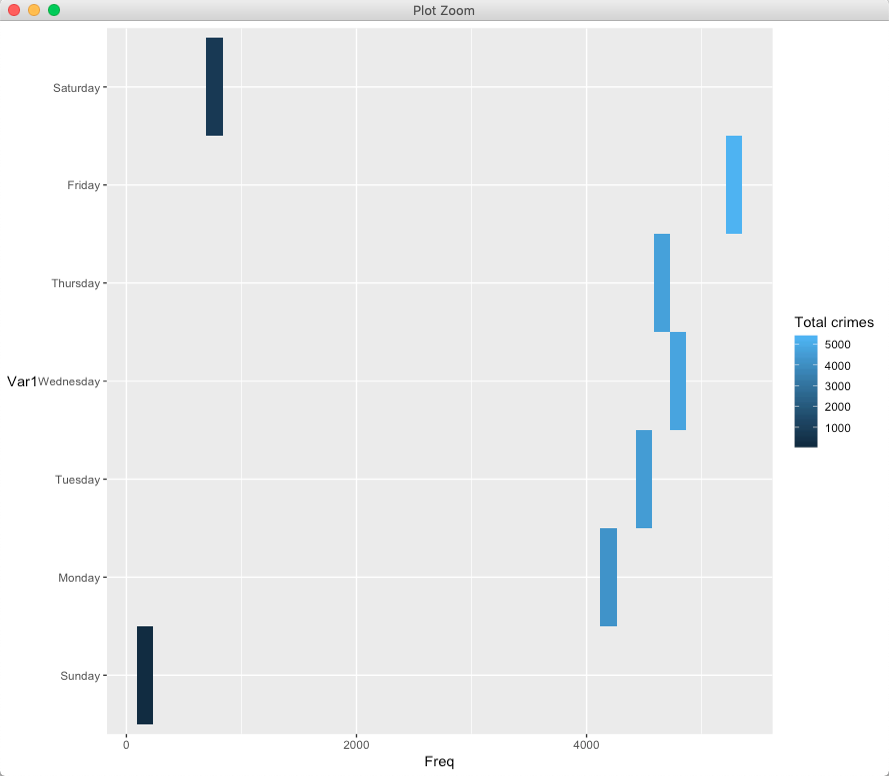
\includegraphics[width=10cm, height = 8cm]{Total_crimes.JPEG}
\end{figure}
\end{frame}
%------------------------------------------------
\begin{frame}{Total Missing Values in \%}
      \begin{figure}        
\centering
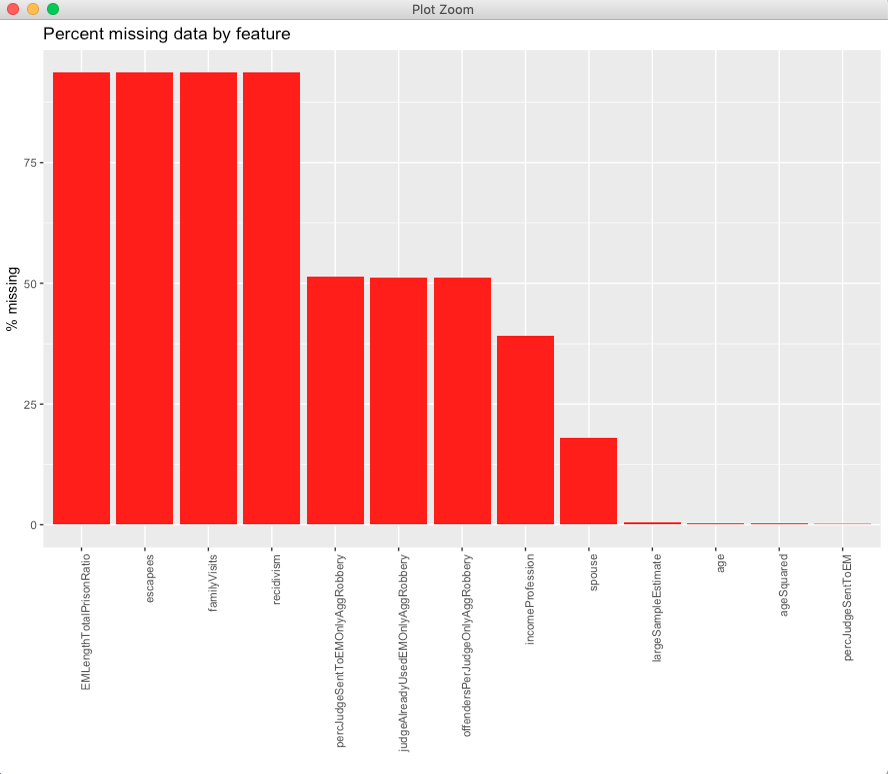
\includegraphics[width=10cm, height = 8cm]{Missing_values.JPEG}
\end{figure}
\end{frame}

%------------------------------------------------
\begin{frame}{Decision Tree}
      \begin{figure}        
\centering
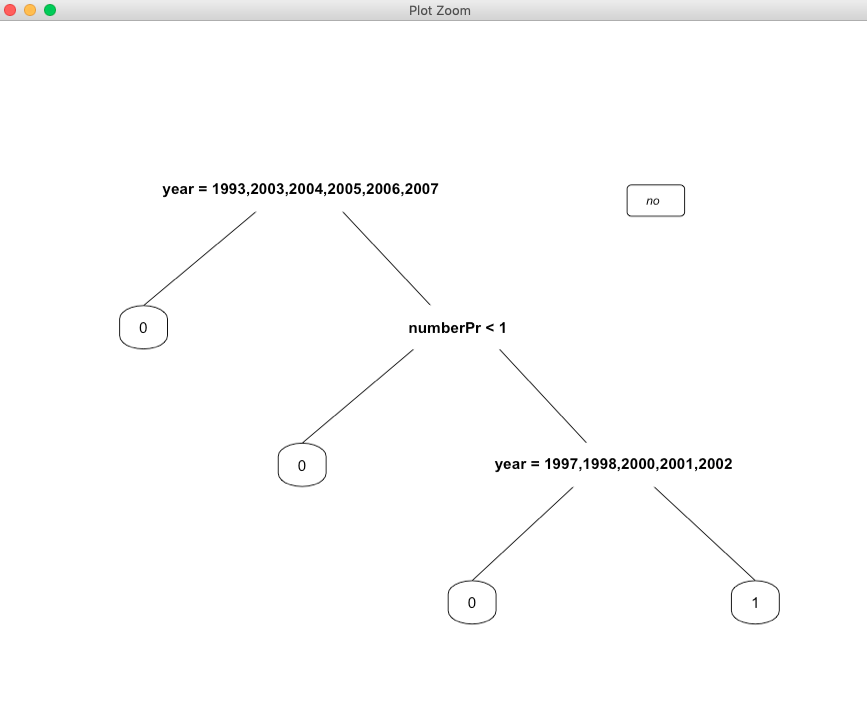
\includegraphics[width=10cm, height = 8cm]{TREE.JPEG}
\end{figure}
\end{frame}

%------------------------------------------------
\begin{frame}{Variable Importance Plot}
      \begin{figure}        
\centering
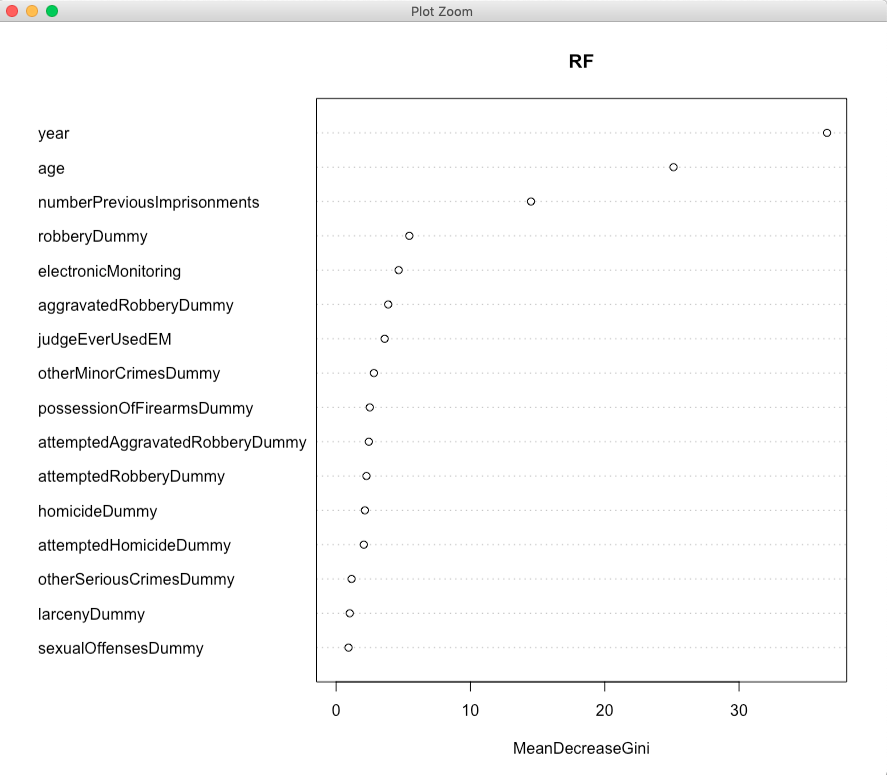
\includegraphics[width=10cm, height = 8cm]{Feature_imp.JPEG}
\end{figure}
\end{frame}
%------------------------------------------------
\begin{frame}
\frametitle{References}
\footnotesize{
\begin{thebibliography}{99} % Beamer does not support BibTeX so references must be inserted manually as below
\bibitem {p1} Di Tella, Schargrodsky (2013)
\newblock Criminal recidivism after Electronic Monitoring and Imprisonment
\newblock \emph{Journal of Political Economy}
\bibitem {p1} Becker (1968)
\newblock Crime and Punishment
\newblock \emph{Journal of Political Economy}
\bibitem {p1} Larsen, Britt (2017)
\newblock Educational Outcomes After Serving with Electronic Monitoring
\newblock \emph{Journal of Quantitative Criminology}
\end{thebibliography}
}


\end{frame}
%------------------------------------------------
\begin{frame}
\Huge{\centerline{Thank you for your attention}}
 \begin{figure}        
\centering

\includegraphics[width=4cm, height = 2.5cm]{github.jpg}
\end{figure}
\end{frame}
%------------------------------------------------
%------------------------------------------------
\end{document}

